\documentclass{article}
\usepackage{leonine,amsmath,amssymb,amsthm,graphicx}
\setkeys{Gin}{width=\linewidth,totalheight=\textheight,keepaspectratio}
\graphicspath{{graphics/}}
% Prints a trailing space in a smart way.
\usepackage{xspace}
% Inserts a blank page
\newcommand{\blankpage}{\newpage\hbox{}\thispagestyle{empty}\newpage}
% \usepackage{units}
% Typesets the font size, leading, and measure in the form of 10/12x26 pc.
\newcommand{\measure}[3]{#1/#2$\times$\unit[#3]{pc}}

\theoremstyle{definition}
\newtheorem{pred}[thm]{Prediction}

\title{Askesis: Introduction} \author{Eric Purdy}

\begin{document}

\maketitle

\section{Perceptron model of a neuron}

A perceptron has two possible outputs, $1$ (representing firing) and
$0$ (representing not firing). Let its inputs be denoted by $x_1,
\dots, x_n$. The rule is then
$$y = \begin{cases} 1 & \sum_i w_i x_i > \theta \\ -1 & \mbox{otherwise}  
\end{cases}$$

The $x_i$ can usually be taken to be either $0$ (if the input neuron
fires) or $1$ (if the input neuron does not fire). Neurons that do not
fire are thus not included in the sum. Occasionally, it is helpful to
think about $x_i$ between zero and one, in which case it can be
encoded by the firing rate. So, if the neuron fires at its maximum
rate, that is represented by a one, and if it doesn't fire at all,
that is represented by a zero. If it fires at a tenth its firing rate,
that is represented by $0.1$.

The $w_i$ are called the synapse weights; each is a summary of
properties of the synapse that occurs between the $i$-th input neuron
and the output neuron. These properties include the physical distance
between the two neurons, as well as the concentration of
neurotransmitter receptors in the output neuron, and other things as
well. If $w_i > 0$, then we call the synapse ``excitatory'' - the
firing of the input neuron excites the output neuron. Most excitatory
synapses use the neurotransmitter glutamate. If $w_i < 0$, we call the
synapse ``inhibitory'' - the firing of the input neuron inhibits the
output neuron. Most inhibitory synapses use the neurotransmitter GABA
(Gamma-Aminobutyric acid). In actual neurons, a single neuron releases
a single main neurotransmitter, and is therefore only ever excitatory
(all synapses it outputs to are excitatory) or inhibitory (all
synapses it outputs to are inhibitory). The parameter $\theta$
controls how excitable the neuron is, and can be modified by
learning. This is called ``intrinsic plasticity''.

\footnote{I like to think of glutamate as the ``black ink'' and GABA as the
  ``red ink'' of the nervous system.}

A perceptron is much simpler than a neuron, but is a reasonable
first-pass approximation. Our model does not require anything more
complicated than perceptrons.

The word ``perceptron'' actually refers to two things: the model
above, and a learning algorithm. We will describe the learning
algorithm here. First, we add an $x_0$ that is always $1$, and let
$w_0 = - \theta$. The perceptron then fires if $\sum_{i=0}^n w_i x_i >
0$. We then suppose that we see a sequence of inputs $x_i(t)$, each
labeled either $1$ or $-1$ by a desired output $\widehat{y}(t)$. The
learning rule is then as follows: if the output $y$ of the neuron was
the same as $\widehat{y}(t)$, we do nothing. If $y(t) \ne
\widehat{y}(t)$, then we update the weights as follows:
$$w_i(t+1) = w_i(t) + \alpha (\widehat{y}(t) - y(t)) x_i(t).$$ If we
start with all $w_i$ equal to zero, then the $w_i(t)$ (considered as a
vector) will be equal to the sum of the $\mathbf{x}(t)$ for which
$\widehat{y}(t)=1,y(t)=0$, minus the sum of the $\mathbf{x}(t)$ for
which $\widehat{y}(t)=0, y(t)=1$. The parameter $\alpha$ is called
the learning rate; high values of $\alpha$ result in a system that
changes its parameters more quickly and thus learns more quickly. A
lower learning rate can be desirable, since the system will be less
likely to lose the information it already has.

The perceptron algorithm is impossible to implement in a single
neuron, since it requires the same synapse to be both excitatory and
inhibitory, depending on what the training data looks like. The
perceptron algorithm is still useful to know, since it can be
implemented by multiple neurons, and has long been thought to be a
large part of how the cerebellum works.


\section{Basic overview of the cerebellum}



\begin{figure}
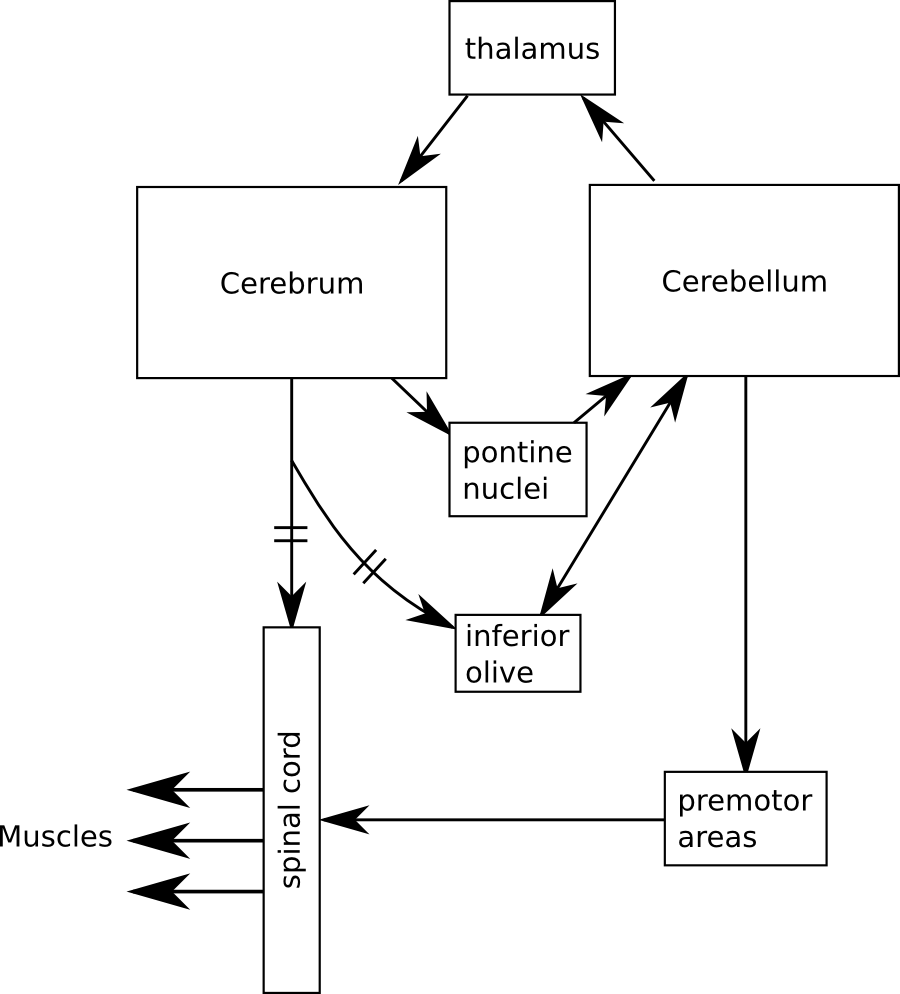
\includegraphics[width=\linewidth]{organization.png}
\caption{Inputs and outputs of the cerebellum. The two arrows marked
  with double lines represent two neural pathways that convey copies
  of the same information.}
\label{fig-organization}
\end{figure}

\begin{figure}
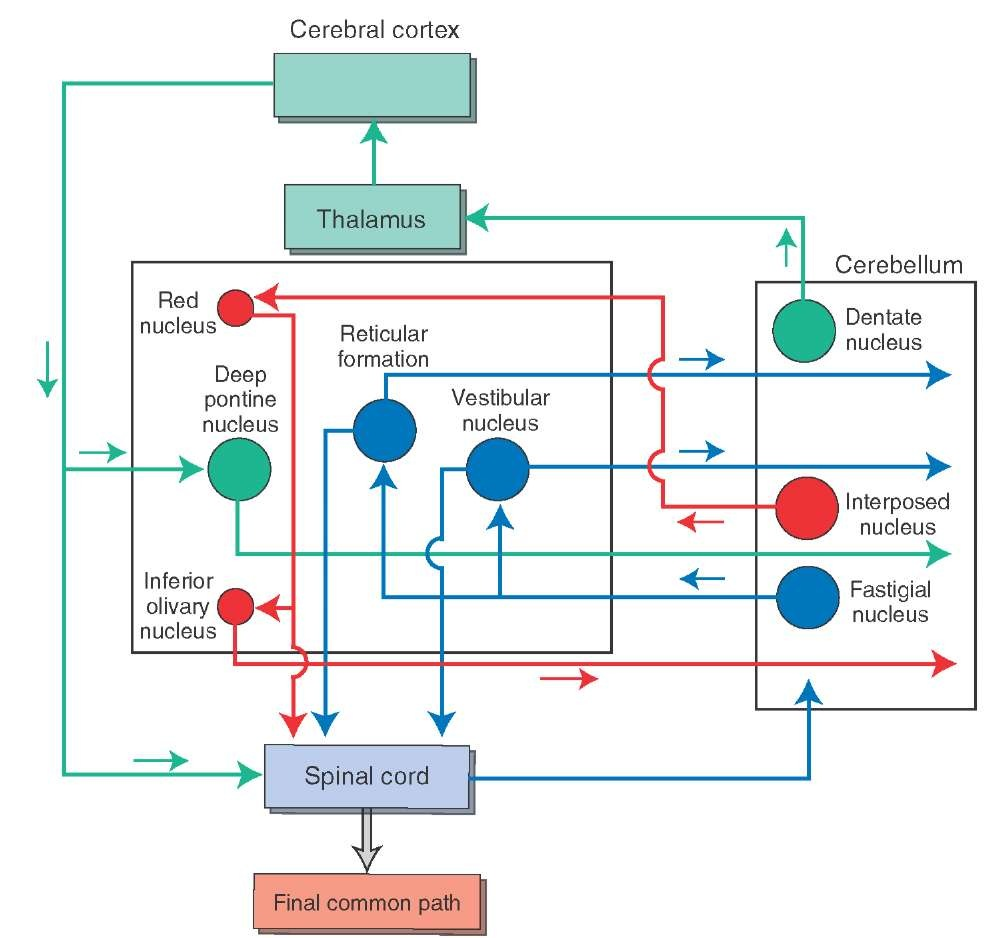
\includegraphics[width=\linewidth]{nanohub/global.png}
\caption{How the cerebellum fits into the rest of the brain. Courtesy
  of
  http://what-when-how.com/wp-content/uploads/2012/04/tmp15F121.jpg}
\label{fig-global}
\end{figure}

\begin{figure}
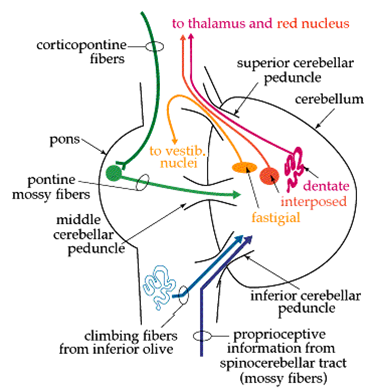
\includegraphics[width=\linewidth]{nanohub/pathways.png}
\caption{Pathways into and out of the cerebellum. The fastigial,
  interposed, and dentate nuclei (and some others) are collectively
  referred to as the deep nuclei, as they lie deep within the
  cerebellum. Courtesy of
  http://www.dizziness-and-balance.com/anatomy/brain/cerebellum.htm}
\label{fig-pathways}
\end{figure}


\section{Cell types}

The cerebellum contains a number of different types of cells:
\begin{description}
\item[Mossy fiber] Mossy fibers are the axons of neurons outside of
  the cerebellum. They constitute one of the two sources of input of
  the cerebellum. One of the major sources of mossy fibers is the
  pontine nuclei, which relay information from the cerebrum.

  All mossy fibers are excitatory. The mossy fibers excite granular
  cells and Golgi cells, and collaterals (side branches) of the mossy
  fibers excite deep nuclear cells.

  Mossy fibers participate in both the positive and negative pathways.

\item[Deep nuclear cell] These are the main source of output from the
  cerebellum. (Some Purkinje cells project to the vestibular nuclei,
  which seem to be pretty similar to the deep nuclei.)

  Some of the deep nuclei are: interposed nucleus, fastigial nucleus,
  dentate nucleus.

  There are two kinds of deep nuclear cell, large and small. The large
  cells can be excitatory or inhibitory, and project to premotor
  areas. The small cells are inhibitory and project to the inferior
  olive.

  Deep nuclear cells receive input from mossy fiber collaterals,
  climbing fiber collaterals, and Purkinje cells.

  Deep nuclear cells participate in both the positive and negative
  pathways.

\item[Inferior olive cell] These are the second source of input to the
  cerebellum. They receive an ``efference'' copy of the signals sent
  from the cerebrum to the spinal cord.

  The inferior olive cells are excitatory and send climbing fibers
  into the cerebellum to make contact with the Purkinje cells,
  stellate cells, and basket cells. A single climbing fiber impulse
  will cause a Purkinje cell to fire. 

  Collaterals of the climbing fiber make contact with the deep nuclear
  cells.

  Inferior olive cells participate in both the positve and negative
  pathways.

\item[Purkinje cell] The Purkinje cells are inhibitory, and send their
  output to the deep nuclear cells. They receive input mainly from the
  parallel fibers, which are the output of the granular cells. They
  also receive some input directly from nearby granular cells.

  Purkinje cells fire at a certain base rate even when not receiving
  any input.

  Purkinje cells participate in the negative pathway.

\item[Basket/stellate cell] Basket and stellate cells inhibit the
  Purkinje cells (and thus disinhibit the deep nuclear cells by
  proxy).

  The stellate cells occupy the outermost portions of the cerebellar
  cortex, while basket cells are slightly more inward. There is also
  an intermediate type of cell that occurs between the basket cells
  and stellate cells and has an appearance halfway between the two.

  Basket and stellate cells participate in the negative pathway.

\item[Granular cell] Granular cells receive input from 4-5 mossy
  fibers. Granular cells are excitatory. The output of the granular
  cell is the parallel fiber, which sends input to the Purkinje cells,
  basket cells, and stellate cells.

  Granular cells are generally thought to fire only when multiple of
  their inputs are active.

  Granular cells are the most numerous neurons in the brain; about
  three-fourths of the neurons in the brain are granular cells in the
  cerebellum. (Granular cells are very small, so the cerebellum only
  takes up about 10\% of the volume of the brain.)

  Granular cells participate in the negative pathway.
\end{description}

\begin{figure}
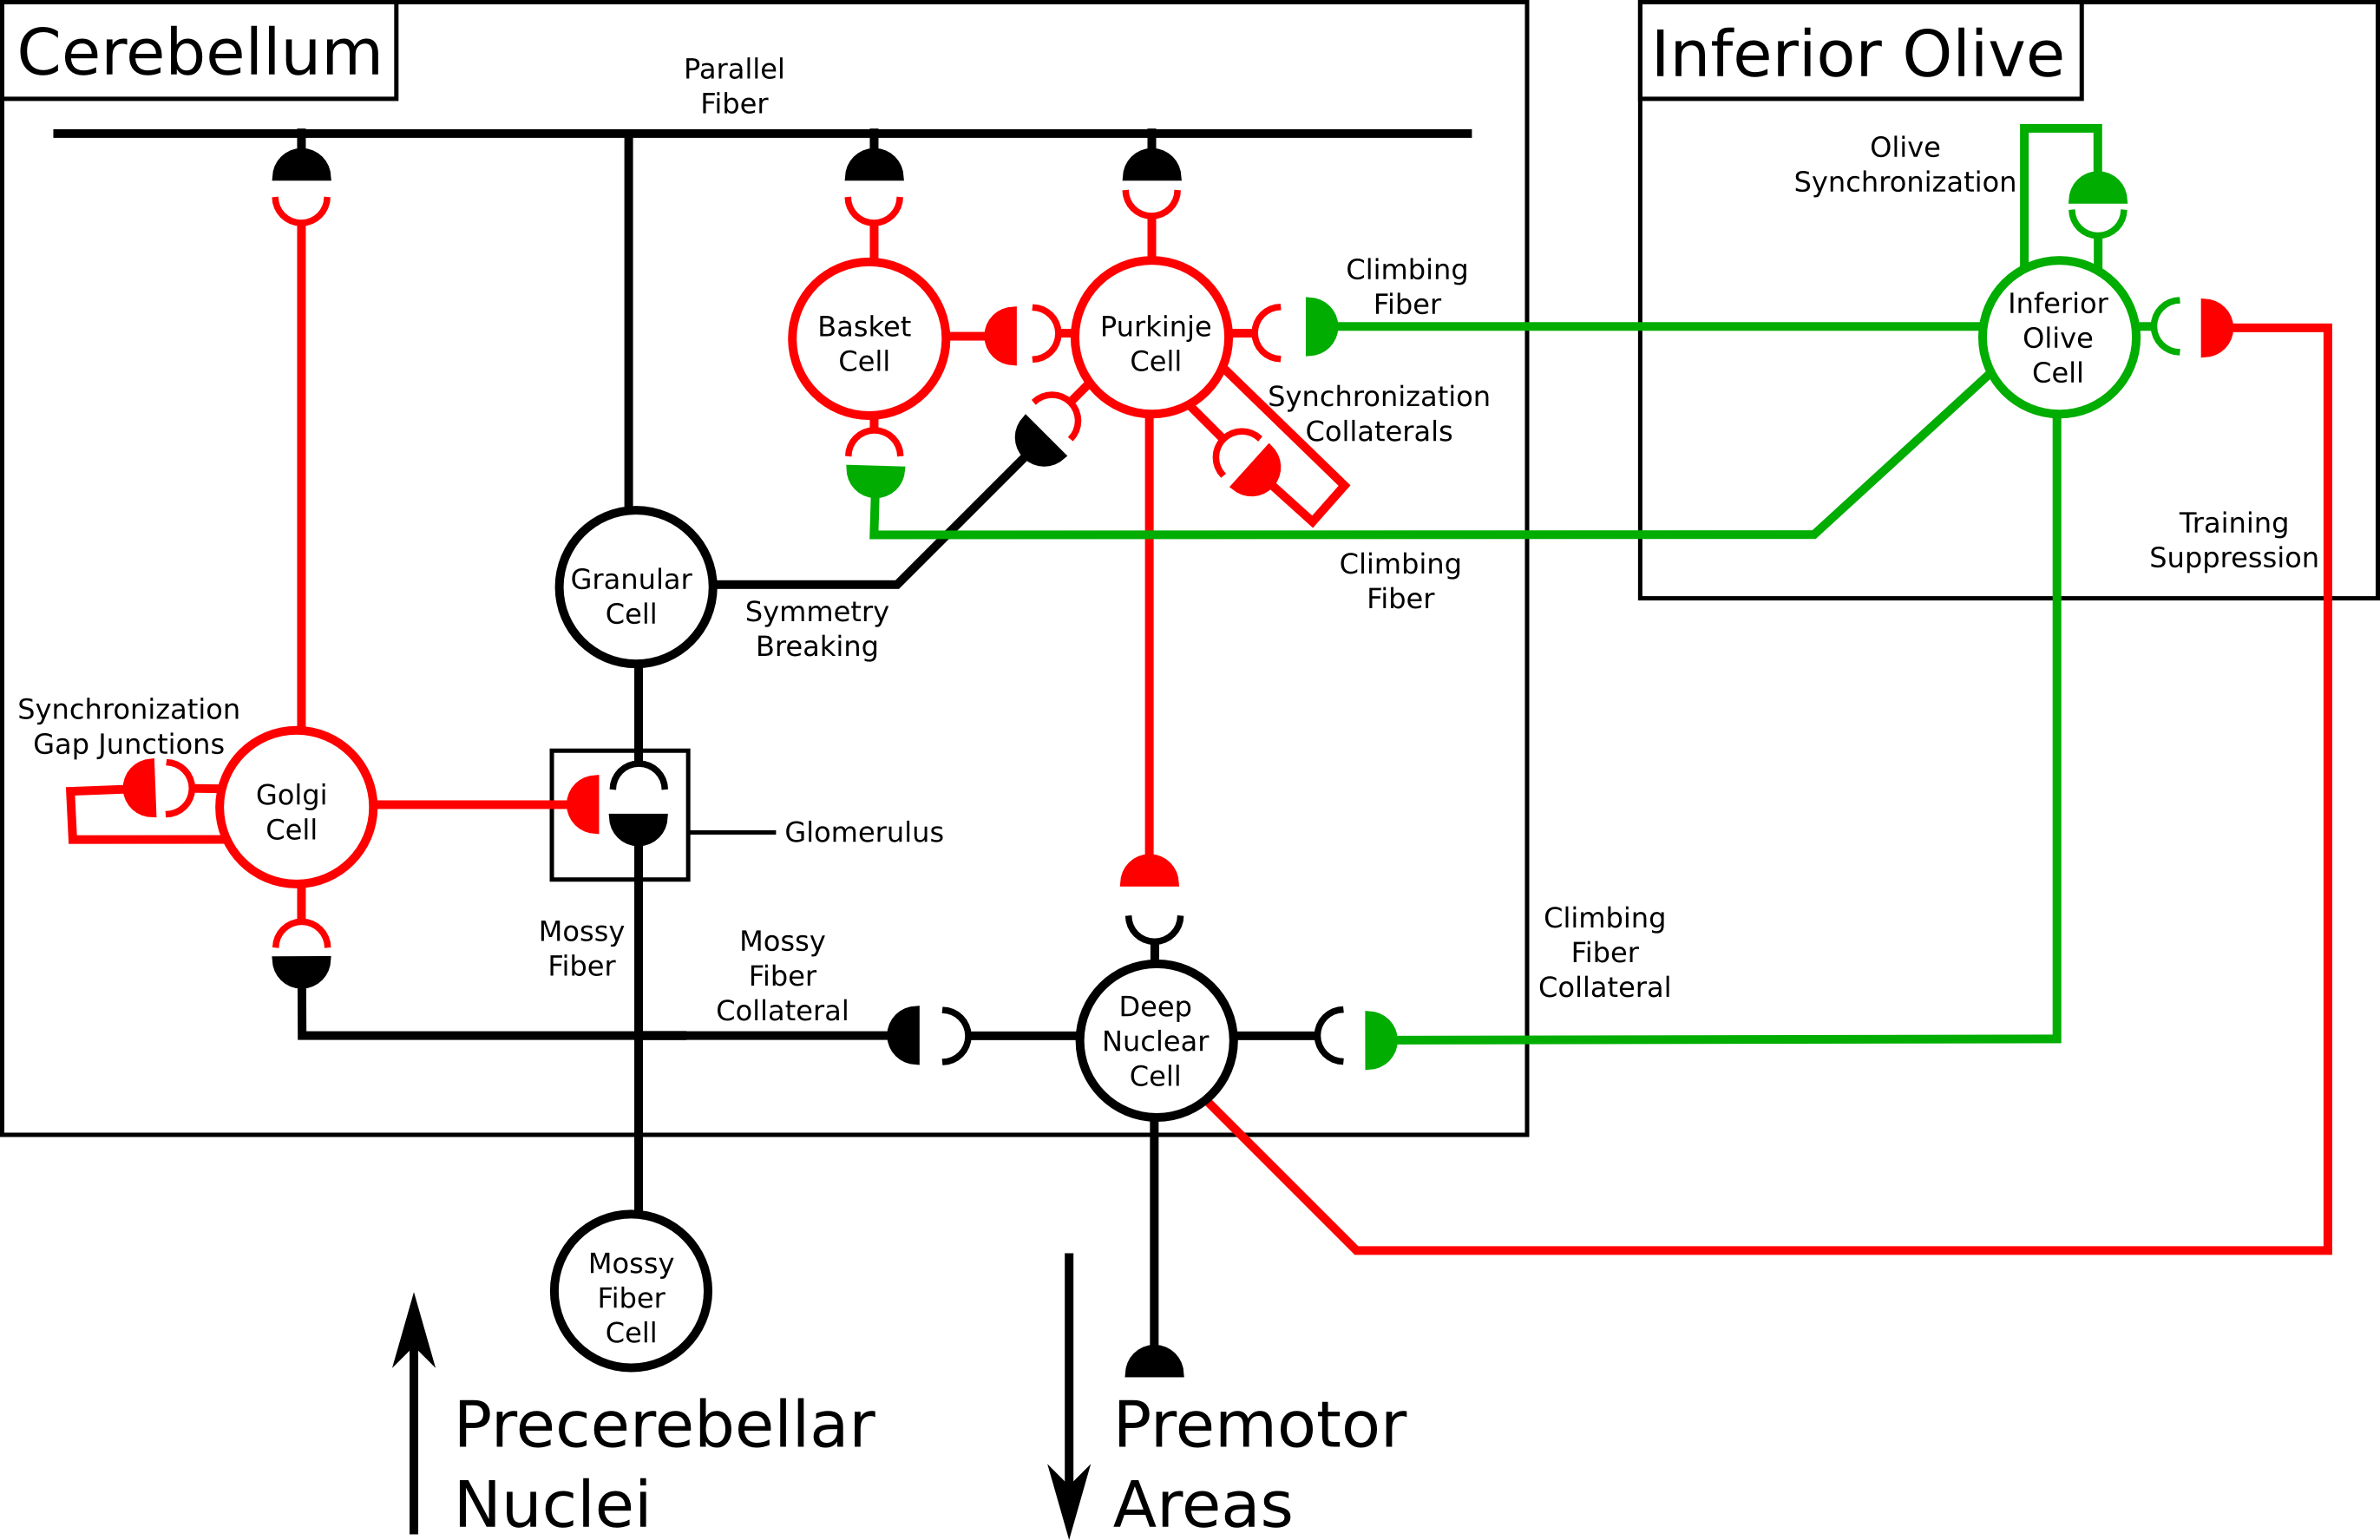
\includegraphics[width=\linewidth]{cells.png}
\caption{Cells of the cerebellum. Excitatory cells are shown in black,
  while inhibitory cells are shown in red. Inputs to a cell are shown
  as an empty half circle, while outputs are shown as a full half
  circle.  Cells of the inferior olive are shown in green, to
  emphasize that their output is used to train the targeted cells;
  they are excitatory. There are two kinds of deep nuclear cell: one
  excitatory and projecting either back into the cerebellum or to
  premotor areas; and one inhibitory and projecting to the inferior
  olive. Since the cells receive the same input, we have simplified
  the picture by identifying them together. It is also worth noting
  that state cells are actually represented twice here: they are both
  ``mossy fiber cells'' and ``deep nuclear cells''.}
\label{fig-cells}
\end{figure}

\begin{figure}
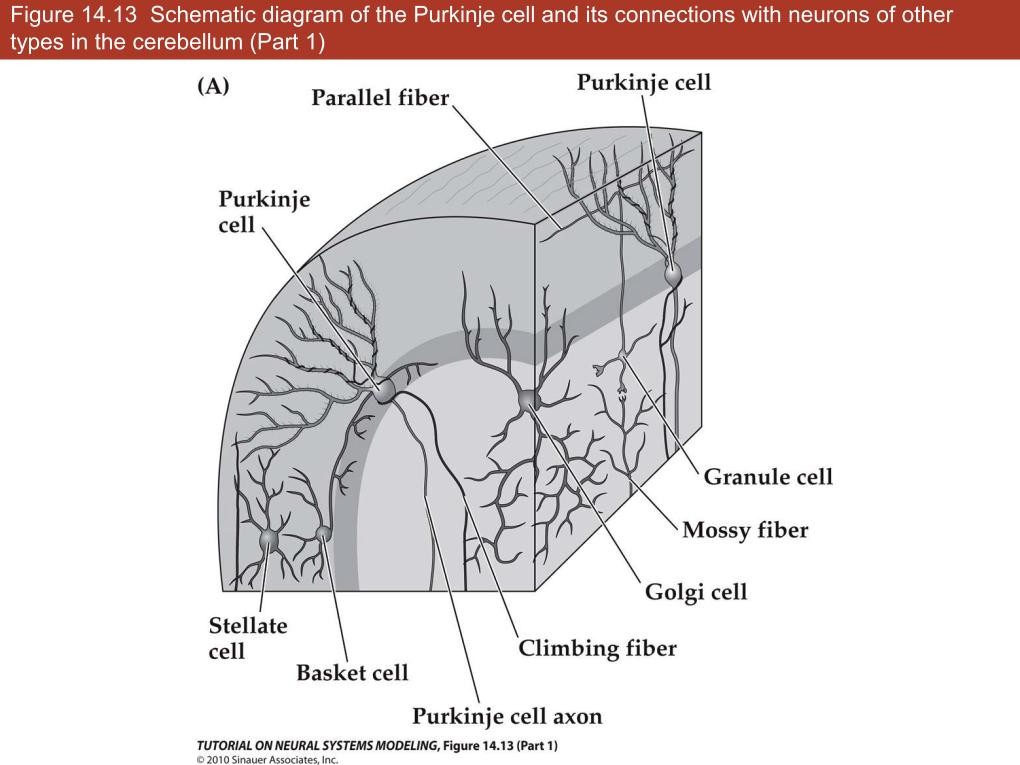
\includegraphics[width=\linewidth]{nanohub/028.png}
\caption{Cells of the cerebellum. Courtesy of
  https://nanohub.org/resources/18948/watch?resid=19060}
\label{fig-physical-1}
\end{figure}

\begin{figure}
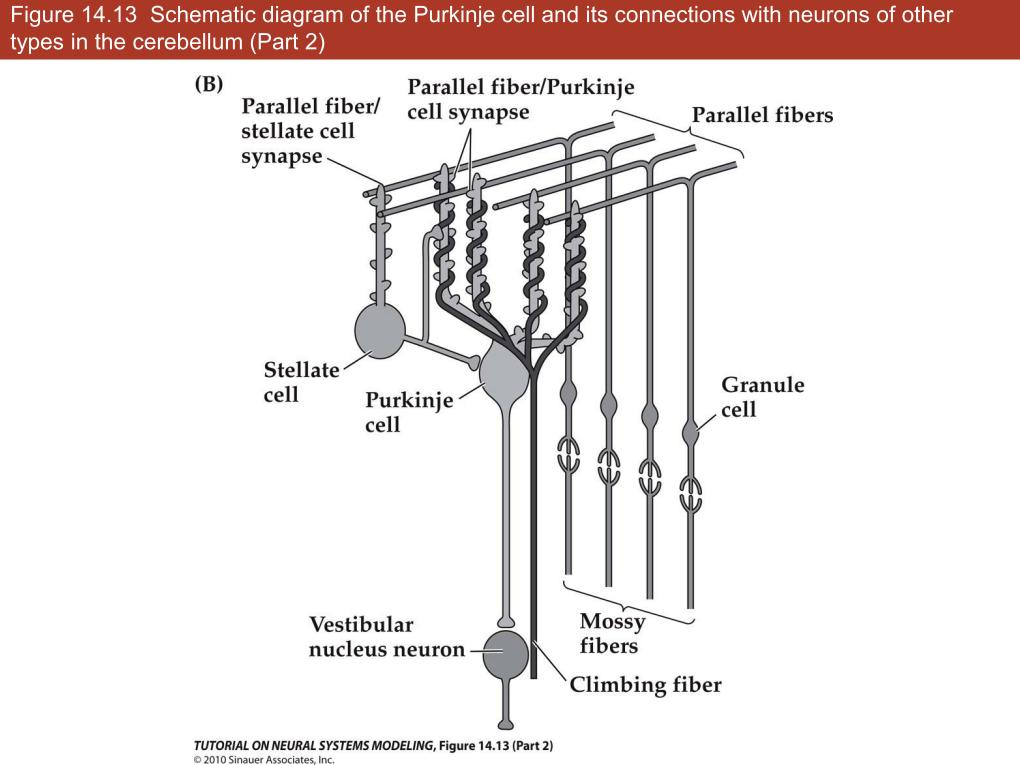
\includegraphics[width=\linewidth]{nanohub/029.png}
\caption{Cells of the cerebellum. Courtesy of
  https://nanohub.org/resources/18948/watch?resid=19060}
\label{fig-physical-2}
\end{figure}

\begin{figure}
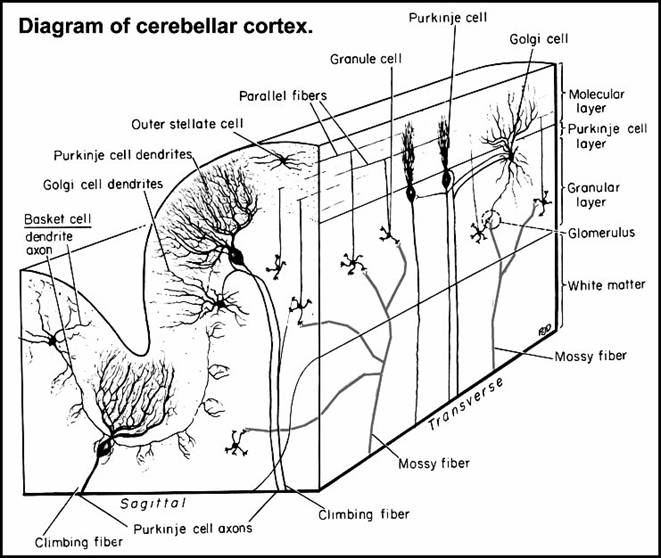
\includegraphics[width=\linewidth]{nanohub/image004.png}
\caption{Cells of the cerebellum. Courtesy of http://www.scritub.com/limba/engleza/health/CEREBELLUM25854.php}
\label{fig-physical-3}
\end{figure}

\begin{figure}
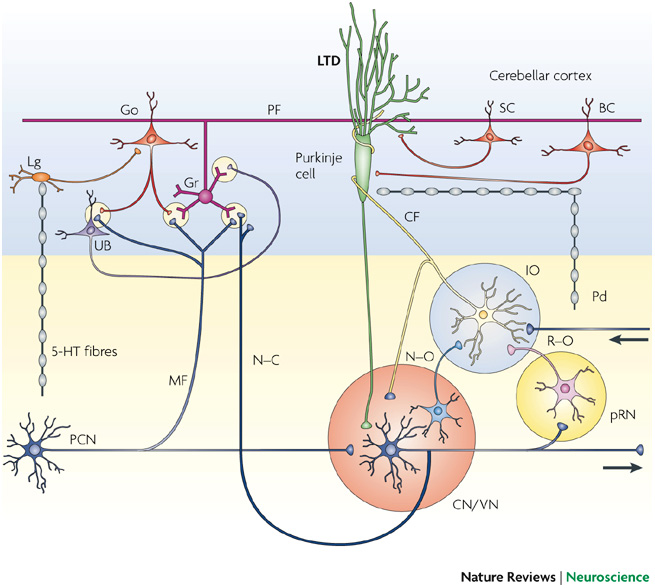
\includegraphics[width=\linewidth]{nanohub/nature.png}
\caption{Cells of the cerebellum. Courtesy of
  http://www.nature.com/nrn/journal/v9/n4/images/nrn2332-f3.jpg.
PCN:pontine nuclei.
MF: mossy fiber.
Lg: Lugaro cell.
5-HT fibres: beaded fibers.
UB: unipolar brush cells (found only in the vestibulocerebellum).
Go: Golgi cell.
Gr: Granular cell.
N-C: state cell pathway.
CN/VN: deep nuclei and vestibular nuclei.
PF: parallel fiber.
LTD: long-term depression, the learning mechanism of the Purkinje cell.
SC: stellate cell.
BC: basket cell.
CF: climbing fiber.
N-O: training suppression cell pathway to inferior olive.
IO: inferior olive.
R-O: red nucleus to inferior olive pathway.
pRN: parvocellular (small cells) red nucleus. 
Pd: unknown, seems to refer to another kind of beaded fiber.
}
\label{fig-physical-4}
\end{figure}


\section{Learning}

As a brief aside to anyone not versed in machine learning or neuroscience,
``learning'' is a term that describes changing the structure or parameters of a
system in order to make that system better achieve some goal or perform some
purpose correctly. The best understood mechanism for learning in the brain is
changing the strength of synapses, the gaps between two neurons, usually by
changing the number of receptors that respond to neurotransmitters.

\section{Thoughts}

\begin{itemize}
\item Discuss microzones. In particular, how big are they? What
  constraints do they impose?
\item Give sigmoid rule with probability.

\item Hebbian learning

\item Explain electrical synapses in the inferior olive?
\end{itemize}

\end{document}
